\documentclass{beamer}
\usepackage[utf8]{inputenc}
\usepackage[T1]{fontenc}
\usepackage{lmodern}  % AMS mathematical facilities for LaTeX.
\usepackage{amsthm}   % Typesetting theorems (AMS style).
\usepackage{amsfonts} % 
\usepackage{mathrsfs}
\usepackage{amsmath,fourier}
\usepackage{amssymb}
\usepackage{cancel}
\usepackage{graphicx}
\usepackage{epsfig}
\usepackage{amsmath,amsfonts,amssymb}
\usepackage{mathpazo}
\usepackage{mathtools}
\theoremstyle{remark}
\newtheorem{remark}{Remark}
\theoremstyle{plain}
\newtheorem{proposition}{Proposition}
\theoremstyle{plain}
\usetheme{Madrid} % Choose a theme (e.g., Madrid, Berlin, etc.)
\usecolortheme{default} % Choose a color theme (e.g., default, albatross, etc.)

% Customize the title page
\title[Spin-0 fields NP constants]{The cylinder at spatial infinity and asymptotic charges}
\author[Rafael Pinto]{Rafael Pinto}
\institute[CENTRA-GRIT]{Instituto Superior Técnico}
\date{\today}
% Add a logo to the title page (optional)
\titlegraphic{
\vspace{-15mm}
\includegraphics[width=1.5cm]{centra.png}
\hspace{\fill}

\includegraphics[width=1.5cm]{grit.png}
}

\begin{document}

% Title Page
\begin{frame}
  \titlepage
  \vfill
  \begin{center}
    Advisors: \textbf{Dr. Edgar Gasper\'in} and \textbf{Dr. Alex Va\~{n}\'o - Vi\~{n}uales}
  \end{center}
\end{frame}

% Table of Contents (optional)
\begin{frame}{Table of Contents}
  \tableofcontents
\end{frame}

% Section 1: Introduction
\section{Newman-Penrose constants}
\begin{frame}{Introduction}
  \begin{itemize}
    \item The Newman-Penrose (NP) constants serve as conserved quantities at null infinity in asymptotically flat gravitational fields.
    \item These constants present a comprehensive conservation system for various spins: spin-1 fields and spin-2 fields, with our research focusing on spin-0 fields linked to wave equation solutions.
    \item In the detailed context, while an infinite series of conserved quantities is identified in the linear theory, the non-linear General Relativity theory conserves only ten.
  \end{itemize}
\end{frame}

\begin{frame}{Conservation laws}
  \begin{itemize}
    \item These charges are computed as 2-surface integrals at cuts ${C} \approx \mathbb{S}^2$ of null infinity $\mathscr{I}$.
  \end{itemize}
  \begin{figure}[h]
    \centering 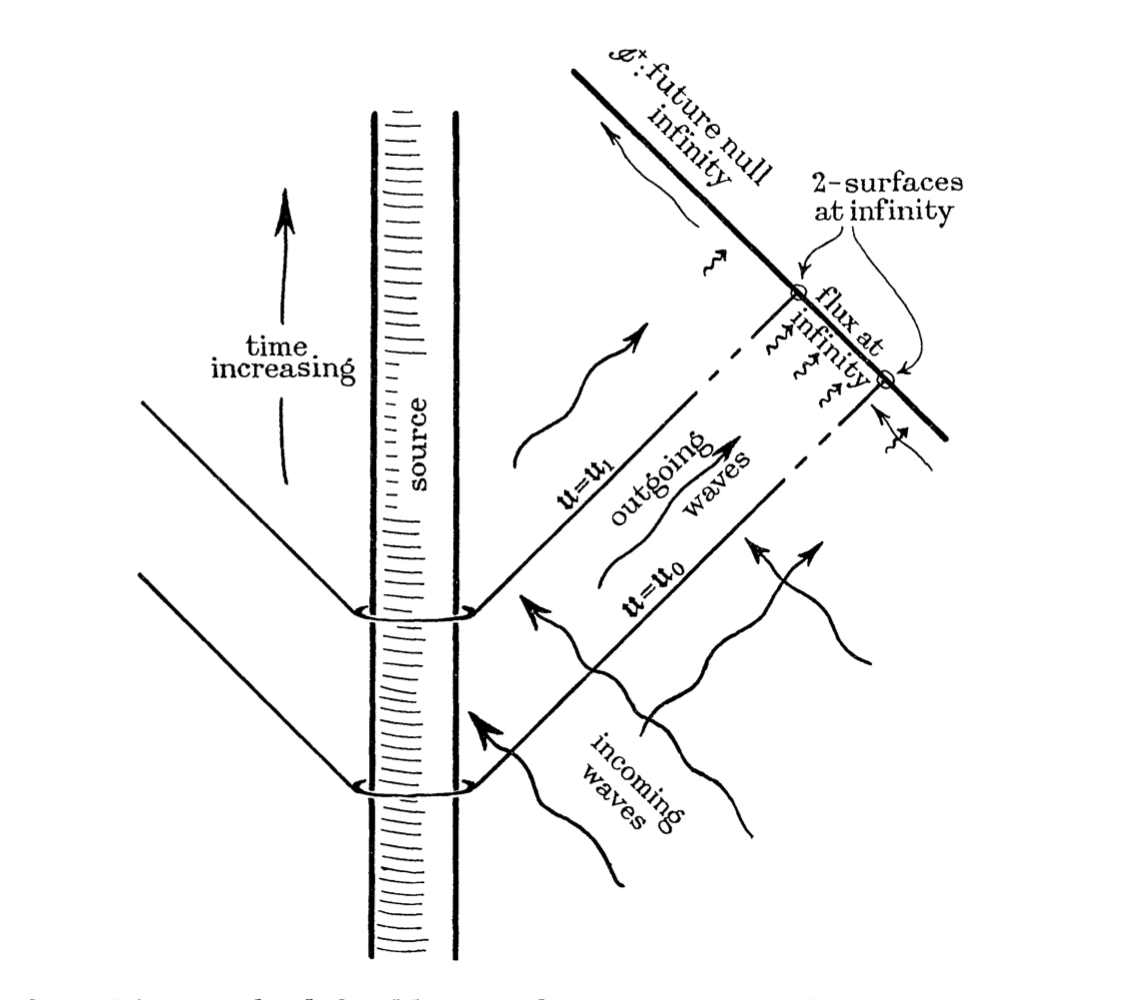
\includegraphics[width =0.45\textwidth]{penrose constants.png}
      \caption{Visual representation of the behavior of the Newman-Penrose constants at null infinity.}
  \end{figure}
\end{frame}
% Section 2: Literature Review
\section{Cylinder at $i^0$}
\begin{frame}{The $i^0$ cylinder representation in Minkowski  spacetime}
  \begin{itemize}
    \item The metric of physical Minkowski spacetime is given by $\tilde{\boldsymbol{\eta}}$:
    \begin{equation}
      \tilde{\boldsymbol{\eta}}=-\mathbf{d} \tilde{t} \otimes \mathbf{d} \tilde{t}+\mathbf{d} \tilde{\rho} \otimes \mathbf{d} \tilde{\rho}+\tilde{\rho}^2 \boldsymbol{\sigma}.
    \end{equation}
    \item The conformal metric in unphysical coordinates, $\boldsymbol{\eta} = \Xi^2 \boldsymbol{\tilde{\eta}}$: 
    \begin{equation}
      \boldsymbol{\eta} = -\frac{1}{\tilde{\rho}^2 - \tilde{t}^2} (-\mathbf{d} \tilde{t} \otimes \mathbf{d} \tilde{t} + \mathbf{d} \tilde{\rho} \otimes \mathbf{d} \tilde{\rho} + \tilde{\rho}^2 \boldsymbol{\sigma}).
    \end{equation}
    \item Introduce coordinates $(\tau, \rho, \vartheta^A)$ with $t = \rho \tau$.
    \item Consider the conformal metric $\boldsymbol{g} = \rho^{-2} \boldsymbol{\eta}$.
    \item Express the unphysical metric $\boldsymbol{g}$ in $F$-coordinates:
    \begin{align}
      & \boldsymbol{g} = -\mathbf{d} \tau \otimes \mathbf{d} \tau + \frac{1 - \tau^2}{\rho^2} \mathbf{d} \rho \otimes \mathbf{d} \rho - \frac{\tau}{\rho} \left(\mathbf{d} \rho \otimes \mathbf{d} \tau + \mathbf{d} \rho \otimes \mathbf{d} \tau\right) + \boldsymbol{\sigma}.
    \end{align}
  \end{itemize}
\end{frame}

\begin{frame}
  \frametitle{Conformal Factor and Lorentz Transformation}
  \begin{itemize}
    \item The conformal factor $\Theta$ in $F$-coordinates and physical coordinates:
    \begin{align}
      \Theta := \rho (1-\tau^2) = \frac{1}{\tilde{\rho}}.
    \end{align}
    \item The boost parameter $\kappa$:
    \begin{align}
      \kappa := \frac{1+\tau}{1-\tau} = -\frac{\tilde{v}}{\tilde{u}}.
    \end{align}
    \item The Lorentz transformation that connects the NP and F-frames:
    \begin{align}
      (\Lambda_{+})^{2} := \Theta^{-1}\kappa^{-1}, \quad (\Lambda_{-})^{2} := \Theta^{-1}\kappa.
    \end{align}
  \end{itemize}
\end{frame}

\begin{frame}
  \frametitle{$i^0$ Cylinder and Null Frames}
  \begin{columns}
    \begin{column}{0.5\textwidth}
      \begin{itemize}
        \item Identify future and past null infinity in the conformal representation:
        \begin{align*}
          \mathscr{I}^{+} & \equiv \{ p \in \mathcal{M} \; \rvert\; \tau(p) =1\}, \\
          \mathscr{I}^{-} & \equiv \{ p \in \mathcal{M} \; \rvert \;\tau(p) =-1\}.
        \end{align*}
        \vspace{0.4cm}
        \item The $i^0$-cylinder represents spatial infinity:
        \begin{align}
          & \mathcal{I} \equiv \{ p \in \mathcal{M} \; \rvert \;\; |\tau(p)| \leq 1, \;\rho(p)=0\}, \\
          & \mathcal{I}^{0} \equiv \{ p \in \mathcal{M}\; \rvert \;\tau(p)=0, \; \rho(p)=0\}.
        \end{align}
      \end{itemize}
    \end{column}
    \begin{column}{0.5\textwidth}
      \vspace*{-6.5em} % Adjust the vertical position as needed
      \hfill
      \begin{figure}[h]
        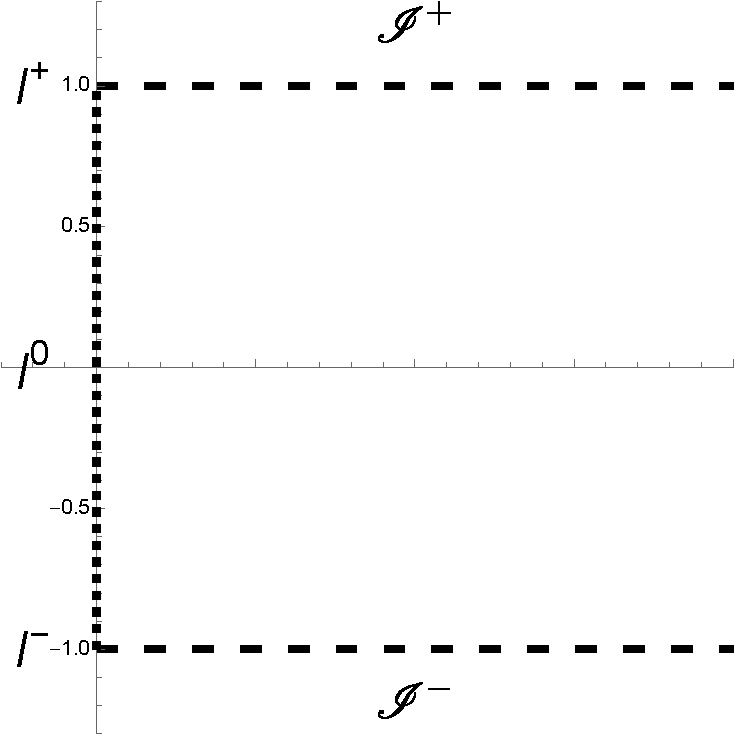
\includegraphics[width=0.7\textwidth]{friedrich cylinder.pdf} % Make sure your file name matches the actual file.
        \caption{Representation of the Friedrich Cylinder.}
      \end{figure}
    \end{column}
  \end{columns}
\end{frame}




\begin{frame}
  \frametitle{$F$-Frame and Null Frames}
  \begin{itemize}
    \item Introduce the $F$-frame:
    \begin{align}
      & \boldsymbol{e}=(1+\tau) \boldsymbol{\partial}_\tau-\rho \boldsymbol{\partial}_\rho, \quad \underline{\boldsymbol{e}}=(1-\tau) \boldsymbol{\partial}_\tau+\rho \boldsymbol{\partial}_\rho, \quad \boldsymbol{e}_{\boldsymbol{A}} \quad \text { with } \nonumber \\ 
      & \boldsymbol{A}=\{\uparrow, \downarrow\}.
    \end{align}
    \item The NP-frame hinged at $\mathscr{I}^{\pm}$:
    \begin{align*}
      \text{NP hinged at} \; \mathscr{I}^{+}: & \quad \boldsymbol{e}^{+}, \underline{\boldsymbol{e}}^{+}, \boldsymbol{e}_{\boldsymbol{A}}^{+}, \\
      \text{NP hinged at} \; \mathscr{I}^{-}: & \quad \boldsymbol{e}^{-}, \underline{\boldsymbol{e}}^{-}, \boldsymbol{e}_{\boldsymbol{A}}^{-}.
    \end{align*}
    \item Transformation between NP and F-frames:
    \begin{align*}
      \text{\emph{NP hinged at} $\mathscr{I}^{+}$}:& \quad\boldsymbol{e}^{+} = \Theta^{-2} L, \quad \underline{\boldsymbol{e}}^{+}= \underline{L},\quad \boldsymbol{e}_{\boldsymbol{A}}^{+}= \boldsymbol{e}_{\boldsymbol{A}}= \Theta^{-1}\tilde{\boldsymbol{e}}_{\boldsymbol{A}}\\ \text{\emph{NP hinged at} $\mathscr{I}^{-}$}:& \quad\boldsymbol{e}^{-} =
       L,\quad \underline{\boldsymbol{e}}^{-}=  \Theta^{-2} \underline{L},\quad \boldsymbol{e}_{\boldsymbol{A}}^{-}= \boldsymbol{e}_{\boldsymbol{A}} = \Theta^{-1}\tilde{\boldsymbol{e}}_{\boldsymbol{A}}.
    \end{align*}
  \end{itemize}
\end{frame}

% Section 3: Methodology
\section{Spin-0 fields close to $i^0$ and $\mathscr{I}$}
\begin{frame}
  \begin{itemize}
    \item For $(\tilde{M},\tilde{\boldsymbol{g}})$ and $(M,\boldsymbol{g})$, the transformation of the D'Alembertian operator under conformal transformations is,
    \begin{equation}\label{eq:waveConfTr}
      \Box \phi-\frac{1}{6} \phi R=\Omega^{-3}\left(\tilde{\Box} \tilde{\phi}-\frac{1}{6} \tilde{\phi} \tilde{R}\right).
    \end{equation}
    \item Using $F$-coordinates, the wave equation is represented by
    \begin{equation}\label{eq:UnphysicalWaveExplicit}
      \left(\tau^2-1\right) \partial_\tau^2 \phi-2 \rho \tau \partial_\tau \partial_\rho \phi+\rho^2 \partial_\rho^2 \phi+2 \tau \partial_\tau \phi+\Delta_{\mathbb{S}^2} \phi=0.
    \end{equation}
    \item We consider the Ansatz
    \begin{equation}\label{eq:ansatz}
      \phi = \sum_{p = 0}^{\infty}\sum_{\ell = 0}^{p}\sum_{m = -\ell}^{m = \ell}\frac{1}{p!}a_{p;\ell,m}(\tau)\rho^{p}Y_{\ell m}.
    \end{equation}
    \item Solving \eqref{eq:UnphysicalWaveExplicit} simplifies to solving the following (ODE) for every $p$, $\ell$, and $m$:
    \begin{equation}\label{eq:ODE_wave_JacobiPoly}
      (1-\tau^2)\ddot{a}_{p;\ell,m} + 2\tau(p-1)\dot{a}_{p,\ell,m}+(\ell+p)(\ell-p+1){a}_{p;\ell,m}=0.
    \end{equation}
  \end{itemize}
\end{frame}

\begin{frame}
  \begin{lemma}\label{Lemma:Sol_Jacobi_and_Logs} The solution to equation \eqref{eq:ODE_wave_JacobiPoly} is given
    by:
    \begin{enumerate}
    \item For $p\geq 1$ and $0\leq \ell \leq p-1$
     \begin{align}\label{eq:Sol_jac_poly}
      & a(\tau)_{p;\ell,m} =A_{p,\ell,m}\bigg(\frac{1-\tau}{2}\bigg)^{p}P_{\ell}^{(p,-p)}(\tau) + \nonumber \\
      & B_{p,\ell,m}\bigg(\frac{1+\tau}{2}\bigg)^{p}P_{\ell}^{(-p,p)}(\tau)
     \end{align}
    
    \item For $p\geq 0$ and $\ell=p$:
       \begin{align}\label{eq:Sol_highestharmonic}
        {a}_{p;p,m}(\tau) =\bigg(\frac{1-\tau}{2}\bigg)^{p}\bigg(\frac{1+\tau}{2}\bigg)^{p}\Bigg(C_{p,p,m}+D_{p,p,m}\int_{0}^{\tau} \frac{ds}{(1-s^2)^{p+1}}\Bigg)
       \end{align}
      \end{enumerate}
  \end{lemma}
\end{frame}

\begin{frame}
  \begin{itemize}
    \item Consider the cases of $p = 0$ and $p = 1$, which yield the following expressions:
    \begin{align}
      {a}_{0;0,0}(\tau) & = C_{000} + \tfrac{1}{2} D_{000} (\log(1 + \tau)- \log(1 - \tau ))\\ 
      {a}_{1;1,m}(\tau) & = \tfrac{1}{4} (1 - \tau )(1 + \tau ) (C_{11m} + \tfrac{1}{4} D_{11m}( \log(1 + \tau ) - \nonumber \\
      & -\log(1 - \tau ) + 2\tau(1-\tau^2))).
    \end{align}
    \item These logarithmic terms have implications for the linear version of the associated peeling property.
    \begin{remark}\label{Remark:logfreeRemark}(Regularity condition).
      \emph{Lemma \ref{Lemma:Sol_Jacobi_and_Logs}} implies that expanding the integral in \eqref{eq:Sol_highestharmonic} results in logarithmic terms, hence $D_{p,p,m} = 0$ is called the regularity condition. The solutions for
      $a(\tau)$ are polynomic in $\tau$, except for $\ell = p$ where one needs to impose the regularity condition to only have polynomic solutions.
    \end{remark}
  \end{itemize}
\end{frame}

\begin{frame}
  \begin{itemize}
    \item We can see how peeling is violated for the spin-0 field by expanding $\tilde{\phi}$ in terms of the $F$-frame:
    \begin{align}\label{eq:phi_tilde}
      & \tilde{\phi}=\frac{C_{000}}{\tilde{\rho}}+\frac{1}{2 \tilde{\rho}} D_{000} \log \left(\frac{\tilde{\rho}+\tilde{t}}{\tilde{\rho}-\tilde{t}}\right) Y_{00} + \frac{1}{8{\tilde{\rho}}}\left(1-\frac{\tilde{t}^{2}}{\tilde{\rho}^{2}}\right) \nonumber \\
      & \left[D_{11-1}\log \left(\frac{\tilde{\rho}+\tilde{t}}{\tilde{\rho}-\tilde{t}}\right) Y_{1-1}+D_{110} \log\left(\frac{\tilde{\rho}+\tilde{t}}{\tilde{\rho}-\tilde{t}}\right) Y_{10}\right] \nonumber \\     
      &+\left[D_{111} \log\left(\frac{\tilde{\rho}+\tilde{t}}{\tilde{\rho}-\tilde{t}}\right)Y_{11}\right]+ \frac{1}{2 \tilde{\rho}}\left(\tilde{t}^{2}-\tilde{\rho}^{2}\right)\left(A_{100}+B_{100}\right) Y_{00}+ \nonumber \\
      &\frac{1}{4 \tilde{\rho}}\left(1-\frac{\tilde{t}^{2}}{\tilde{\rho}^{2}}\right)\left(C_{11-1} Y_{1-1}+C_{110} Y_{10}+C_{111} Y_{11}\right).
    \end{align}
    \item In the spin-0 case, the peeling property is violated by the logarithmic terms that appear in the expansion of $\tilde{\phi}$.
  \end{itemize}
\end{frame}
% Section 4: Results
\section{The NP-constants for the spin-0 fields close to $i^0$ \& $\mathscr{I}$}
\begin{frame}{The NP-constants for the spin-0 fields close to $i^0$ \& $\mathscr{I}$}
  \begin{itemize}
    \item Conservation laws:
    \begin{equation}\label{eq:cons_laws}
      {\underline{{L}}}({\tilde{\rho}}^{-2\ell}L(e^{+})^{\ell+1}\phi_{\ell m})=0, \qquad L({\tilde{\rho}}^{-2\ell}\underline{L}(e^{-})^{\ell+1}\phi_{\ell m})=0
    \end{equation}
    \item One can introduce the $f(\tilde{\rho})$-modified NP constants in the following manner: 
    \begin{align}\label{eq:DefModifiedNP}
      {}^{f}\mathcal{N}^{+}_{\ell,m}:= f(\tilde{\rho})L (\boldsymbol{e}^{+})^{\ell}\phi_{\ell m} \Big|_{{C}^{+}}, \\ 
      {}^{f}\mathcal{N}^{-}_{\ell,m}:= f(\tilde{\rho})\underline{L} (\boldsymbol{\underline{e}}^{-})^{\ell}\phi_{\ell m}\Big|_{{C}^{-}}.
    \end{align}
    \item For $f(\tilde{\rho})=\tilde{\rho}^2$, these quantities are referred to as the "classical NP-constants" and are denoted as $\mathcal{N}^{\pm}_{\ell,m}$.
    \begin{align}\label{eq:classicalNP}
      \mathcal{N}^{+}_{\ell,m}:= (\boldsymbol{e}^{+})^{\ell+1}\phi_{\ell m}\Big|_{{C}^{+}},\\ 
      \mathcal{N}^{-}_{\ell,m}:= (\boldsymbol{\underline{e}}^{-})^{\ell+1}\phi_{\ell m} \Big|_{{C}^{-}}.
    \end{align}
  \end{itemize}
\end{frame}
% Section 5: Conclusion
\section{The classical NP constants at $\mathscr{I}^{+}$}
\begin{frame}{The classical NP constants at $\mathscr{I}^{+}$}
  \begin{itemize}
    \item This analysis is facilitated by the expression,
    \begin{align}\label{eq:exp_phi_lm}
      \phi_{\ell m}= \sum_{p=\ell}^{\infty}\frac{1}{p!}a_{p;\ell,m}(\tau)\rho^{p}.
    \end{align}
    \item Considering $\ell=0$, the computation of $\boldsymbol{e}^{+}(\phi_{00})$ is sufficient.
    \begin{align}\label{eq:bmeplus1philmraw}
      & \boldsymbol{e}^{+}(\phi_{\ell m}) = 4 \rho^{-1}(1+\tau)^{-2}\sum_{p=0}^{\infty} \frac{1}{p!}\rho^p((1+\tau)\dot{a}_{p;\ell,m}-p a_{p;\ell,m}).
    \end{align}
    With
    \begin{align}\label{eq:defQ0}
      Q^{0}_{p;\ell,m}(\tau):=(1+\tau)\dot{a}_{p;\ell,m}-p a_{p;\ell,m}.
    \end{align}
    \item With this definition in place, we can express $\boldsymbol{e}^{+}(\phi_{\ell m})$ as follows:
    \begin{align}\label{eq:bmeplus1philm}
      \boldsymbol{e}^{+}(\phi_{\ell m}) = 4 (\Lambda_{+})^{2}\sum_{p=0}^{\infty} \frac{1}{p!}\rho^{p}Q^{0}_{p,\ell,m}(\tau).
    \end{align}
  \end{itemize}
\end{frame}

\begin{frame}
  \begin{itemize}
    \item To compute the $\ell=0$ NP constant at $\mathscr{I}^{+}$, it is necessary to evaluate $\boldsymbol{e}^{+}(\phi_{00})$ at a specific cut ${C}^{+}$ of $\mathscr{I}^{+}$. By utilizing equation \eqref{eq:bmeplus1philm} we obtain the following expression:
    \begin{align}
      \mathcal{N}^{+}_{0,0}= \lim_{\substack{\rho \to \rho_{\star} \\ \tau \to 1}}  \boldsymbol{e}^{+}(\phi_{00}) =\sum_{p=0}^{\infty} \frac{1}{p!}\rho^{p-1}_{\star}Q^{0}_{p,0,0}|_{\mathscr{I}^{+}} = -A_{100}.
    \end{align}
    \item To calculate the $\ell = 1$ NP constants, one has\\
    \begin{align}
      \mathcal{N}^{+}_{1,m} = \lim _{\substack{\rho \rightarrow 0 \\ \tau \rightarrow 1}}2^{-4} \frac{1}{2 !} Q^{1}_{2, 1, m}\cdot(\tau) = 3A_{21m}.
    \end{align}
    \item The NP constants for $\mathscr{I}^{-}$ can be calculated in a similar manner, where the time reversed version of the $F$-frame is used.
  \end{itemize}
\end{frame}

\section{The $i^0$ cylinder logarithmic NP constants at $\mathscr{I}^{-}$}
\begin{frame}{The $i^0$ cylinder logarithmic NP constants at $\mathscr{I}^{-}$}
  \begin{itemize}
    \item Choice of $f(\tilde{\rho})$.
    \item The constants $D_{p;\ell,m}$ that define the regularity condition precisely correspond to the $f(\tilde{\rho}) = \tilde{\rho}$-modified NP constants.
    \item We will compute the $\ell=0$ and $\ell=1$ modified NP constants ${}^{f}\mathcal{N}^{-}_{\ell,m}$.
    \begin{align}
      \tilde{\rho}\underline{L} (\phi_{\ell m}) = \frac{(1+\tau)}{(1-\tau)}\sum_{p=0}^{\infty}\underline{Q}^{0}_{p;\ell,m}(\tau)\rho^p.
    \end{align}
    Therefore, for $\ell=0$, we have:
    \begin{align}
      \mathcal{}^{\tilde{\rho}}\mathcal{N}^{-}_{0,0} = \lim_{\substack{\rho \to \rho_{\star} \\ \tau \to -1}} \; \kappa(\underline{\boldsymbol{e}^{-}})(\phi_{00}) = \sum_{p=0}^{\infty}\rho_{\star}^p\biggl[\frac{(1+\tau)}{(1-\tau)}\underline{Q}^{0}_{p;0,0}\biggr]|_{\mathscr{I}^{-}}.
    \end{align}
  \end{itemize}
\end{frame}

\begin{frame}
  \begin{itemize}
    \item Evaluating at the critical set $\mathcal{I}^{-}$, we obtain:
    \begin{align}
      \mathcal{}^{\tilde{\rho}}\mathcal{N}^{-}_{0,0} = \lim_{\substack{\rho \to \rho_{\star} \\ \tau \to -1}}\sum_{p=0}^{\infty}\rho_{\star}^p\biggl[\frac{(1+\tau)}{(1-\tau)}\underline{Q}^{0}_{p;0,0}\biggr] = \frac{1}{2}D_{000}.
    \end{align}
    \item Similarly, for $\ell=1$, the relevant quantity to evaluate is:
    \begin{align}
      \tilde{\rho} \underline{L} (\underline{\boldsymbol{e}^{-}}) \phi_{1m}= 4\kappa(\Lambda_{-})^{2}\sum_{p=1}^{\infty}\frac{1}{p!}\rho^p\underline{Q}^{1}_{p;\ell,m}.
    \end{align}
    \item Therefore, for $\ell=1$, we have:
    \begin{align}
      \mathcal{}^{\tilde{\rho}}\mathcal{N}^{-}_{1,m} = \lim_{\substack{\rho \to \rho_{\star} \\ \tau \to -1}} \; \kappa\underline{\boldsymbol{e}}(\underline{\boldsymbol{e}^{-}})\phi_{1m} = \sum_{p=1}^{\infty}\frac{1}{p!}\rho_{\star}^{p-1}(\kappa \underline{Q}^{1}_{p;1,m})|_{\mathscr{I}^{-}}.
    \end{align}
    \item Evaluating at the critical set $\mathcal{I}^{-}$, we obtain:
    \begin{align}
      \mathcal{}^{\tilde{\rho}}\mathcal{N}^{-}_{1,m} = - \frac{1}{4}D_{11m}.
    \end{align}
  \end{itemize}
\end{frame}

\section{The NP constants in terms of initial data}
\begin{frame}{The NP constants in terms of initial data}
  \begin{itemize}
    \item Classical NP Constants at $\mathscr{I}^{+}$: $\mathcal{N}^{+}_{\ell,m} = q^{+}(\ell) \;A_{\ell+1,\ell,m}$.
    \item Modified NP Constants at $\mathscr{I}^{+}$: ${}^{\tilde{\rho}}\mathcal{N}^{+}_{\ell,m} = q^{+}(\ell) \;D_{\ell,\ell,m}$.
    \item Classical NP Constants at $\mathscr{I}^{-}$: $\mathcal{N}^{-}_{\ell,m} = q^{-}(\ell) \; B_{\ell+1,\ell,m}$.
    \item Modified NP Constants at $\mathscr{I}^{-}$: ${}^{\tilde{\rho}}\mathcal{N}^{-}_{\ell,m} = q^{-}(\ell) \;D_{\ell,\ell,m}$.
    \item Key Observations for Spin-0 Field Near $i^0$:
    \begin{enumerate}
      \item Regularity condition is essential for well-defined NP constants.
      \item Classical NP constants differ between $\mathscr{I}^{\pm}$.
      \item Logarithmic NP constants at $\mathscr{I}^{\pm}$ are equivalent (up to a numerical constant) with the same initial data.
    \end{enumerate}
  \end{itemize}
\end{frame}
% References (optional)
\section{Conclusions}
\begin{frame}{Conclusions}
  \begin{itemize}
    \item Computed the NP constants for a spin-0 field near spatial and null infinity using the \(i^0\) cylinder framework, exploring the link between NP constants at future and past null infinity based on initial data. 
    \item Analytic initial data prescribed near \(i^0\) results in solution irregularity at the convergence sets \(\mathcal{I}^{\pm}\), controlled by a constant \(D_{p;p,m}\). 
    \item When the regularity condition, \(D_{p;p,m} = 0\), is unmet, the classical NP constants become undefined, allowing a polyhomogeneous expansion for the physical field \(\tilde{\phi}\) around null infinities. 
    \item Upon satisfying the regularity condition, the classical NP constants at \(\mathscr{I}^{\pm}\) arise from unique initial data components. 
    \item Conclusively, while classical NP constants at \(\mathscr{I}^{\pm}\) usually lack correspondence, the \(i^0\) cylinder NP constants at \(\mathscr{I}^{\pm}\) consistently align due to shared origins in the initial data.
  \end{itemize}
\end{frame}
\end{document}
